\section{Grundlagen}


\Term{Mikrostreifenleitungen}:
Quasi-TEM-Wellen
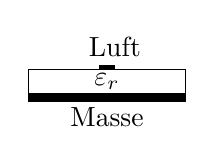
\begin{tikzpicture}
    \draw (0,0) rectangle (2,0.3) node[midway] {$\varepsilon_r$};
    \filldraw (0,0) rectangle (2,-0.1) node[midway, below] {Masse};
    \filldraw (0.9,0.3) rectangle (1.1,0.35) node[at end, above] {Luft};
\end{tikzpicture}

\Term{Triplate Leitung}:
TEM-Wellen

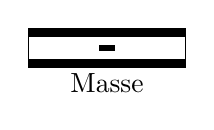
\begin{tikzpicture}
    \draw (0,0) rectangle (2,0.3);
    \filldraw (0,0) rectangle (2,-0.1) node[midway, below] {Masse};
    \filldraw (0,0.3) rectangle (2,0.4);
    \filldraw (0.9,0.12) rectangle (1.1,0.18);
\end{tikzpicture}




\Term{Leitungsgleichung}
$\gamma, Z_L$

$U = U_f \e^{- \gamma z} + U_b \e^{\gamma z}$
$I = \frac{U_f}{Z_L} \e^{-\gamma z} - \frac{U_f}{Z_L} \e^{\gamma z}$

Normierungs:

$u = \frac{U}{\sqrt{Z_L}}$ , $i = I \sqrt{Z_0}$ , $U_f = I_f Z_L$

$u = u_f\e^{-\gamma z} + u_b\e^{\gamma z} = a + b$\\
$i = a-b$


\Term{Matrixbeschreibungen}
\begin{pitemize}
    \item \Term{S-Parameter (Streuparameter)}:
    \begin{pitemize}
        \item Beschreibung über Wellen ($a_i$ (Eingang Oben), $b_i$ (Ausgang unter), Nummer sind die Seite)
        \item $\begin{pmatrix} b_1 \\ b_2 \end{pmatrix}
                =
                \begin{pmatrix} S_{11} & S_{12} \\ S_{21} & S_{22} \end{pmatrix}
                \begin{pmatrix} a_1 \\ a_2 \end{pmatrix}$
            \begin{pitemize}
                \item $S_{11} \big|_{a_2 = 0} = \frac{b_1}{a_1}$: Reflexion Eingang
                \item $S_{21} \big|_{a_2 = 0} = \frac{b_2}{a_1}$: Transmission (Verstärkung)
                \item $S_{12}$: Rückwirkung
                \item $S_{22}$: Reflexion Ausgang
            \end{pitemize}
    \end{pitemize}

    \item \Term{Impedanzparameter}:
    \begin{pitemize}
        \item $U_1 = Z_{11}I_1 + Z_{12}I_2$
        \item $U_2 = Z_{21}I_2 + Z_{22}I_2$
    \end{pitemize}

    \item \Term{T-Parameter (ABCD-Parameter)}:
    \begin{pitemize}
        \item Zusammenhang von Spannungen und Strömen
        \item Ideal für Kaskadierung (Matrizenmultiplikation)
        \item $\begin{pmatrix} U_1 \\ I_1 \end{pmatrix}
            =
            \begin{pmatrix} A & B \\ C & D \end{pmatrix}
            \begin{pmatrix} U_2 \\ -I_2 \end{pmatrix}$
    \end{pitemize}


    \item \Term{Kettenparameter}:
    \begin{pitemize}
        \item Alternative Darstellung der ABCD-Parameter
        \item $\begin{pmatrix} U_1 \\ I_1 \end{pmatrix}
            =
            \begin{pmatrix} A & B \\ C & D \end{pmatrix}
            \begin{pmatrix} U_2 \\ I_2 \end{pmatrix}$
    \end{pitemize}
\end{pitemize}
